
\documentclass[]{report}
\voffset=-1.5cm
\oddsidemargin=0.0cm
\textwidth = 480pt


\usepackage{amsmath}
\usepackage{graphicx}
\usepackage{amssymb}
\usepackage{framed}
\usepackage{multicol}
%\usepackage[paperwidth=21cm, paperheight=29.8cm]{geometry}
%\usepackage[angle=0,scale=1,color=black,hshift=-0.4cm,vshift=15cm]{background}
%\usepackage{multirow}
\usepackage{enumerate}

\usepackage{amsmath,amsfonts,amssymb}
\usepackage{color}
\usepackage{multirow}
\usepackage{eurosym}
\usepackage{framed}

%\input def.tex
%\input dsdef.tex
%\input rgb.tex

%\newcommand \la{\lambda}
%\newcommand \al{a}
%\newcommand \be{b}
\newcommand \x{\overline{x}}
\newcommand \y{\overline{y}}

\begin{document}
%============================================%
\subsection{3.6 Refinements of the concept of Nash equilibrium}
We consider 3 refinements of the concept of Nash equilibrium,
which are useful when there are multiple equilibria.
\begin{enumerate}
	\item Subgame perfect Nash equilibria.
	\item Payoff dominant Nash equilibria.
	\item Risk domninant Nash equilibria.
\end{enumerate}

%%- 32 / 61
%============================================%
%=================================================%
\subsection{Subgame Perfect Equilibria in the Context of Matrix Games}
\begin{itemize}
	\item We have considered the concept of subgame perfection in extended
	games.
	\item In the asymmetric Hawk-Dove game, Player 1 will take action H
	and Player 2 will take action D under the following strategy pairs
	(H, [D|H, H|D]) and (H, [D|H, D|D]).
	\item 	However, when Player 2 plays [D|H, D|D] he does not use his best
	response when Player 1 makes a ”mistake” and plays D. Hence,
	the second pair of actions does not define a subgame perfect Nash
	equilibrium.
	\item 	We will now consider the matrix form of this game (this was
	derived earlier).
\end{itemize}

%%- 33 / 61
%============================================%
\subsubsection{Subgame Perfect Equilibria in the Context of Matrix Games}
%(H|H, H|D) (H|H, D|D) (D|H, D|D) (D|H, H|D)
%H (-2,-2) (-2,-2) (4,0) (4,0)
%D (0,4) (2,2) (2,2) (0,4)

\begin{figure}[h!]
\centering
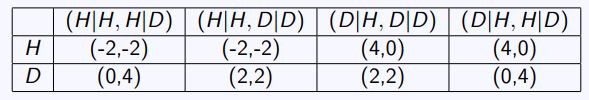
\includegraphics[width=0.7\linewidth]{images/DR6-Slide34}
\caption{}
\label{fig:DR6-Slide34}
\end{figure}

It can be seen that (H, [D|H, D|D]) is a (weak) Nash equilibrium
in this game, since neither player can increase their payoff by
unilaterally switching strategy.
%%- 34 / 61
%============================================%

%Subgame Perfect Equilibria in the Context of Matrix Games
\begin{itemize}
	\item However, the strategy [D|H, H|D] dominates the action
	[D|H, D|D], since Player 2 always does as well by playing
	[D|H, H|D] rather than [D|H, D|D] and does better when Player 1
	plays D.
	\item 	It can be shown that (H, [D|H, H|D]) is the only Nash equilibrium
	left after the removal of dominated strategies.
\end{itemize}

%% 35 / 61
%============================================%
\subsection{Payoff Dominant Nash Equilibria}
\begin{itemize}
	\item A payoff vector (v1, v2) is said to Pareto dominate payoff vector
	(x1, x2) if v1 ≥ x1, v2 ≥ x2 and inequality is strict in at least one of
	the cases.
	\item	That is to say, Nash Equilibrium 1 of a game Pareto dominates
	Nash Equilibrium 2 if no player prefers Equilibrium 1 to Equilibrium
	2 and at least one player prefers Equilibrium 1.
	\item	A Nash equilibrium is payoff dominant if the value of the game
	corresponding to this equilibrium Pareto dominates all the values
	of the game corresponding to other equilibria.
\end{itemize}

%%- 36 / 61
%============================================%
%=================================================%
\subsection{Example}
Consider the following game
A B
A (4,4) (0,0)
B (0,0) (2,2)
Such a game is called a coordination game, as both players would
like to take the same action.
%%- 37 / 61
%============================================%
%=================================================%
\subsection{Example}
There are 3 Nash equilibria
1. (A, A) - Value (4,4).
2. (B, B) - Value (2,2).
3. (1/3A + 2/3B, 1/3A + 2/3B) - Value ( 4
3
,
4
3
).
The first equilibrium Pareto dominates the other two equilibria,
whilst the second equilibrium Pareto dominates the third.
(A, A) is the payoff dominant equilibrium.
%%- 38 / 61
%============================================%
\subsection{Risk Dominance}
\begin{itemize}
	\item Suppose there are pure Nash equilibria (A, C) and (B, D).
	\item The risk factor associated with strategy A, FA, is the probability
	with which Player 2 should play C (which is used at the Nash
	equilibrium where Player 1 plays A), in order to make Player 1
	indifferent between playing A or B.
	\item 	A high risk factor indicates that Player 1 must be relatively sure
	that Player 2 will play C for Player 1 to prefer A to B.
	\item 	Similarly, the risk factor associated with strategy B is the
	probability with which Player 2 should play D, in order to make
	Player 1 indifferent between playing A or B.
\end{itemize}

%%- 39 / 61
%============================================%
%%- \subsection{Risk Dominance}
\begin{itemize}
	\item The risk factors associated with C and D can be calculated in a
	similar way.
	\item The Nash equilibrium (A, C) risk dominates (B, D) if FA ≤ FB ,
	FC ≤ FD and there is strictly inequality in at least one case.
\end{itemize}

%%- 40 / 61
%============================================%
\subsection{Example}
Consider the following symmetric game
A B
A (4,4) (-1000,0)
B (0,-1000) (2,2)
It is clear that the equilibrium (A, A) payoff dominates the
equilibrium (B, B). However, there is a large risk associated with
playing action A (the possibility of obtaining a payoff of -1000).
%% 41 / 61
%=================================================%
%% \subsection{Example}
From the symmetry of the game, the risk factors of the two
strategies are the same for both players.
The risk factor associated with A is given by the solution of
4p − 1000(1 − p) = 0p + 2(1 − p) ⇒ p =
1002
1006
.
The risk factor associated with B is given by the solution to
2p + 0(1 − p) = −1000p + 4(1 − p) ⇒ p =
4
1006
.
It follows that B risk dominates A.
%% 42 / 61
%============================================%
\subsection{Conclusion}
\begin{itemize}
	\item If an equilibrium both payoff and risk dominates another, it seems
	clear that this should be the one chosen.
	\item In other cases, it is not clear what equilibrium should be played.
	\item The concept of risk domination is important in evolutionary game
	theory (see later).
\end{itemize}

%%- 43 / 61
%============================================%
%=================================================%
\subsection{3.7 2-Player Games with a Continuum of Strategies and
Simultaneous Moves}
\begin{itemize}
	\item Assume that Player i chooses an action from a finite interval Si
	.
\item The payoff to Player i when Player 1 takes action x1 and Player 2
	takes action x2 is given by Ri(x1, x2).
\item It is assumed that the payoff functions are differentiable.
\end{itemize}

%%- 44 / 61
%============================================%
\subsection{The Symmetric Cournot Game}
\begin{itemize}
\item Assume that two firms produce an identical good. Firm i produces
xi units per time interval.
\item The price of the good is determined by total supply and all
production is sold at this ”clearing price”. It is assumed that
p = A − B[x1 + x2], (A, B > 0).
\item The costs of producing x units of the good are assumed to be
C + Dx for both firms.
\item The payoff of a firm is taken to be the profit obtained (revenue
minus costs). Revenue is simply production times price.
\end{itemize}

%% 45 / 61
%============================================%
\subsection{The Symmetric Cournot Game}
The payoff obtained by Firm 1 is given by
\[R1(x1, x2) = px1 − C − Dx1 = (A − D)x1 − Bx2
1 − Bx1x2 − C.\]
By symmetry, the payoff obtained by Player 2 is
\[R2(x1, x2) = px2 − C − Dx2 = (A − D)x2 − Bx2
2 − Bx1x2 − C.\]
It should be noted that it clearly does not pay firms to produce
more than the amount xmax that guarantees that the price is equal
to the unit (marginal) cost of production. Since xmax is finite, we
may assume that firms choose their strategy (production level)
from a finite interval.
%% 46 / 61
%============================================%
\subsection{Best Response Functions}
Given the output of the opponent, we can calculate the optimal
response of a player using calculus.
Let B1(x2) denote the best response of Player 1 to x2.
Let B2(x1) denote the best response of Player 2 to x1.
47 / 61
Nash Equilibria in Games with a Continuum of Strategies
and Simultaneous Actions
At a Nash equilibrium (x
∗
1
, x
∗
2
), we have
x
∗
1 = B1(x
∗
2
); x
∗
2 = B2(x
∗
1
).
Thus, at a Nash equilibrium Player 1 plays her best response to
Player 2’s strategy and vice versa.
%%- 48 / 61
%============================================%
\subsection{The Cournot Game}
Suppose A = 3, B =
1
1000 , C = 100 and D = 1.
We have
R1(x1, x2) = 2x1 −
x
2
1
1000
−
x1x2
1000
− 100.
In order order to derive the best response of Player 1 to Player 2’s
action, we differentiate Player 1’s payoff function with respect to
x1, his action.
%%- 49 / 61
%============================================%
%%- \subsection{The Cournot Game}
We have
\[∂R1(x1, x2)
∂x1
= 2 −
2x1 + x2
1000
.\]
It should be noted that this derivative is decreasing in x1, hence
any stationary point must be a maximum.
The optimal response is given by
2 −
2x1 + x2
1000
= 0 ⇒ x1 = 1000 −
x2
2
.
Thus B1(x2) = 1000 −
x2
2
.
%% 50 / 61
%============================================%
\subsection{The Cournot Game}
It should be noted that this solution is valid as long as x2 ≤ 2000
(production cannot be negative).
If x2 > 2000, then ∂R1(x1,x2)
∂x1
is negative for all non-negative values
of x1.
In this case the best response is not to produce anything.
%%- 51 / 61
%============================================%
%%- \subsection{The Cournot Game}
By symmetry the best response of Player 2 is given by
B2(x1) = max{0, 1000 −
x1
2
}.
We look for an equilibrium at which both firms are producing. In
this case
x
∗
1 = 1000 −
x
∗
2
2
; x
∗
2 = 1000 −
x
∗
1
2
.
It follows that at Nash equilibrium both firms must produce 2000
3
units.
Intuitively, from the form of the game both firms should produce
the same amount.
%%- 52 / 61
%=================================================%
%%- \subsection{The Cournot Game}
The value of the game can be found by substituting these values
into the payoff functions.
R1(x
∗
1
, x
∗
2
) = R2(x
∗
1
, x
∗
2
) = 2 ×
2000
3
− 2 ×
1000
9
− 100 ≈ 344.
The equilibrium price is 3 − 2 ×
2
3 =
5
3
.
%%- 53 / 61
%============================================%
\subsection{The Cournot Game}
\begin{itemize}
	\item There cannot be an equilibrium at which one of the firms does not
	produce. The argument is as follows.
	\item If one firm does not produce, then the optimal response to this is
	to produce 1000 units.
	\item (0,1000) cannot be a Nash equilibrium, since the best response of
	Firm 1 to x2 = 1000 is to choose x1 = 500.
\end{itemize}

%%- 54 / 61
%============================================%
\section{The Stackelberg Model}
\begin{itemize}
	\item This is identical to the Cournot model, except that it is assumed
	that one of the firms is a market leader and chooses its production
	level before the second firm chooses.
	\item	The second firm observes the production level of the first.
\end{itemize}

%%- 55 / 61
%============================================%
\subsection{Games with a Continuum of Strategies and Sequential Moves}
\begin{itemize}
\item Suppose Player 2 moves after Player 1 and observes the action
taken by Player 1. The equilibrium is derived by recursion.
\item Player 2 should choose the optimum action given the action of
Player 1.
\item Hence, we first need to solve
∂R2(x1, x2)
∂x2
= 0.
\item This gives the optimal response of Player 2 as a function of the
strategy of Player 1, x2 = B2(x1).
\end{itemize}

%%- 56 / 61
%============================================%
\subsection{Games with a Continuum of Strategies and Sequential  Moves}

\begin{itemize}
	\item We now calculate the optimal strategy of the first player to move.
	\item If Player 1 plays x1, Player 1 responds by playing B2(x1). Hence,
	we can express the payoff of Player 1 as a function simply of x1,
	i.e. R1(x1, B2(x1)).
	\item 	In order to find the optimal action of Player 1, we differentiate this
	function with respect to x1.
	\item 	Having calculated the optimal value of x1, we can derive x2.
\end{itemize}

%%- 57 / 61
%============================================%
\subsection{Example}
Derive the equilibrium of the Stackelberg version of the previous
example.
We have
R2(x1, x2)=2x2 −
x
2
2
1000
−
x1x2
1000
− 100.
∂R2(x1, x2)
∂x2
=2 −
x2
500
−
x1
1000
.
%%- 58 / 61
%============================================%
\subsection{Example}
It follows that the best response of Player 2 is given by
2 −
x2
500
−
x1
1000
= 0 ⇒ x2 = 1000 −
x1
2
.
Hence,
R1(x1, B2(x1))=R1(x1, 1000 −
x1
2
)
=2x1 −
x
2
1
1000
−
x1(1000 − x1/2)
1000
− 100
=x1 −
x
2
1
2000
− 100.

\begin{figure}[h!]
\centering
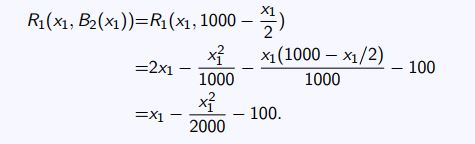
\includegraphics[width=0.7\linewidth]{images/DR6-Slide59}
\caption{}
\label{fig:DR6-Slide59}
\end{figure}

%%- 59 / 61
%============================================%
\subsection{Example}
Differentiating
\[∂R1(x1, B2(x1))
∂x1
= 1 −
x1
1000
.\]
It follows that Firm 1 maximises its profit by producing 1000 units.
The best response of Firm 2 is B2(x1) = 1000 −
x1
2 = 500 units.
\begin{itemize}
	\item The Stackelberg equilibrium is (1000, 500).
	\item Hence, the leader
	produces more than at the Cournot equilibrium and the follower
	produces less.
\item Total production is greater than at the Cournot equilibrium, i.e.
	the equilibrium price is lower.
\end{itemize}

%% 60 / 61
%============================================%
\subsection{Example}
The profit of Firm 1 at this equilibrium is
\[R1(1000, 500) = 2 × 1000 − 1000 − 500 − 100 = 400.\]
The profit of Firm 2 at this equilibrium
\[R2(1000, 500) = 2 × 500 − 250 − 500 − 100 = 150.\]
It is clear that Firm 1 gains by being the leader. Firm 2 loses. The
sum of profits is lower than at the Cournot equilibrium.
This seems somewhat counter-intuitive, as the market would seem
to be more competitive under the Cournot model.
%% 61 / 61


\end{document}